In this section, we give a brief introduction about the state-of-the-art supervised bug localization NPCNN (Natural and Programming language Convolutional Neural Network), which was proposed by Huo et al.~\cite{huo2016learning}. %Our model is built on NPCNN for cross-project bug localization.

The goal of supervised bug localization is training prediction model using bug reports and source code,  and then predicts the localization of buggy code that produces the program behaviors specified in a given bug report. Let $\mathcal{C} =\{ c_1, c_2, \cdots, c_{n_1} \}$ denotes a set of source code, and $\mathcal{R} =\{ r_1, r_2, \cdots, r_{n_2}\} $ denotes a set of bug reports, where $n_1, n_2$ denote the number of source files and bug reports from source and target project, respectively. We formulate a cross-project bug localization as a learning task which aims to learn a prediction function $f: \mathcal{R} \times \mathcal{C} \mapsto \mathcal{Y}$. $y_{ij} \in \mathcal{Y} = \{+1, -1 \}$ indicates whether a source code $c_j \in \mathcal{C} $ is relevant to a bug report $r_i \in \mathcal{R}$.

Noticing that semantics of bug reports in natural language and source code in programming language are different, the NPCNN model employs separate Convolutional Neural Networks (CNNs) for semantic features from bug reports and source code. The general structure of NPCNN is illustrated in Figure~\ref{fig:npcnn-structure}. Bug reports and source code are first encoded as one-hot feature vectors and then fed into the CNNs. In the intra-language feature extraction layers, two CNNs are employed for semantic feature extraction: CNN for natural language follows standard approach~\cite{kim2014convolutional}, and CNN for programming language is specifically designed. 

\begin{figure}[hbt]
\centering
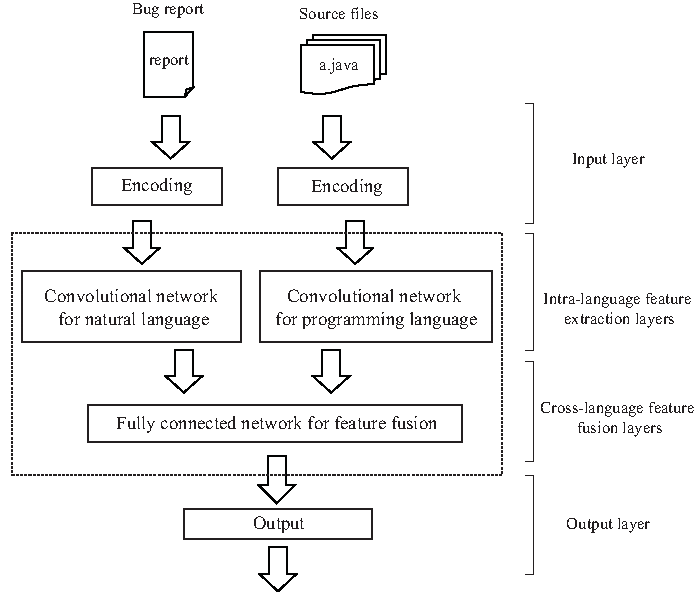
\includegraphics[width = \columnwidth]{pic/NPCNN-structure.pdf}
\caption{The general structure of Natural and Programming language Convolutional Neural Network.}
\label{fig:npcnn-structure}
\end{figure}

Huo et al.~\cite{huo2016learning} found that programming language%, although in textual format,
differs from natural language in two aspects. First, the basic language component carrying meaningful semantics in natural language is word or term, while the basic language component carrying meaningful semantics in programming language is statement. Second, natural language organizes words in a ``flat'' way while programming language organizes its statements in a ``structured'' way to produce richer semantics. Therefore, the structure of CNN for programming language, as shown in Figure~\ref{fig:npcnn}, is specifically designed to solve these two points. The first convolutional and pooling layers extract within-statements features while preserving the integrity of statements by sliding convolutional window within statements. The subsequent convolutional and pooling layers extract between-statements features reflecting the structural nature by employing different size of convolutional windows. More details can be referred to in~\cite{huo2016learning}.

\begin{figure}[hbt]
\centering
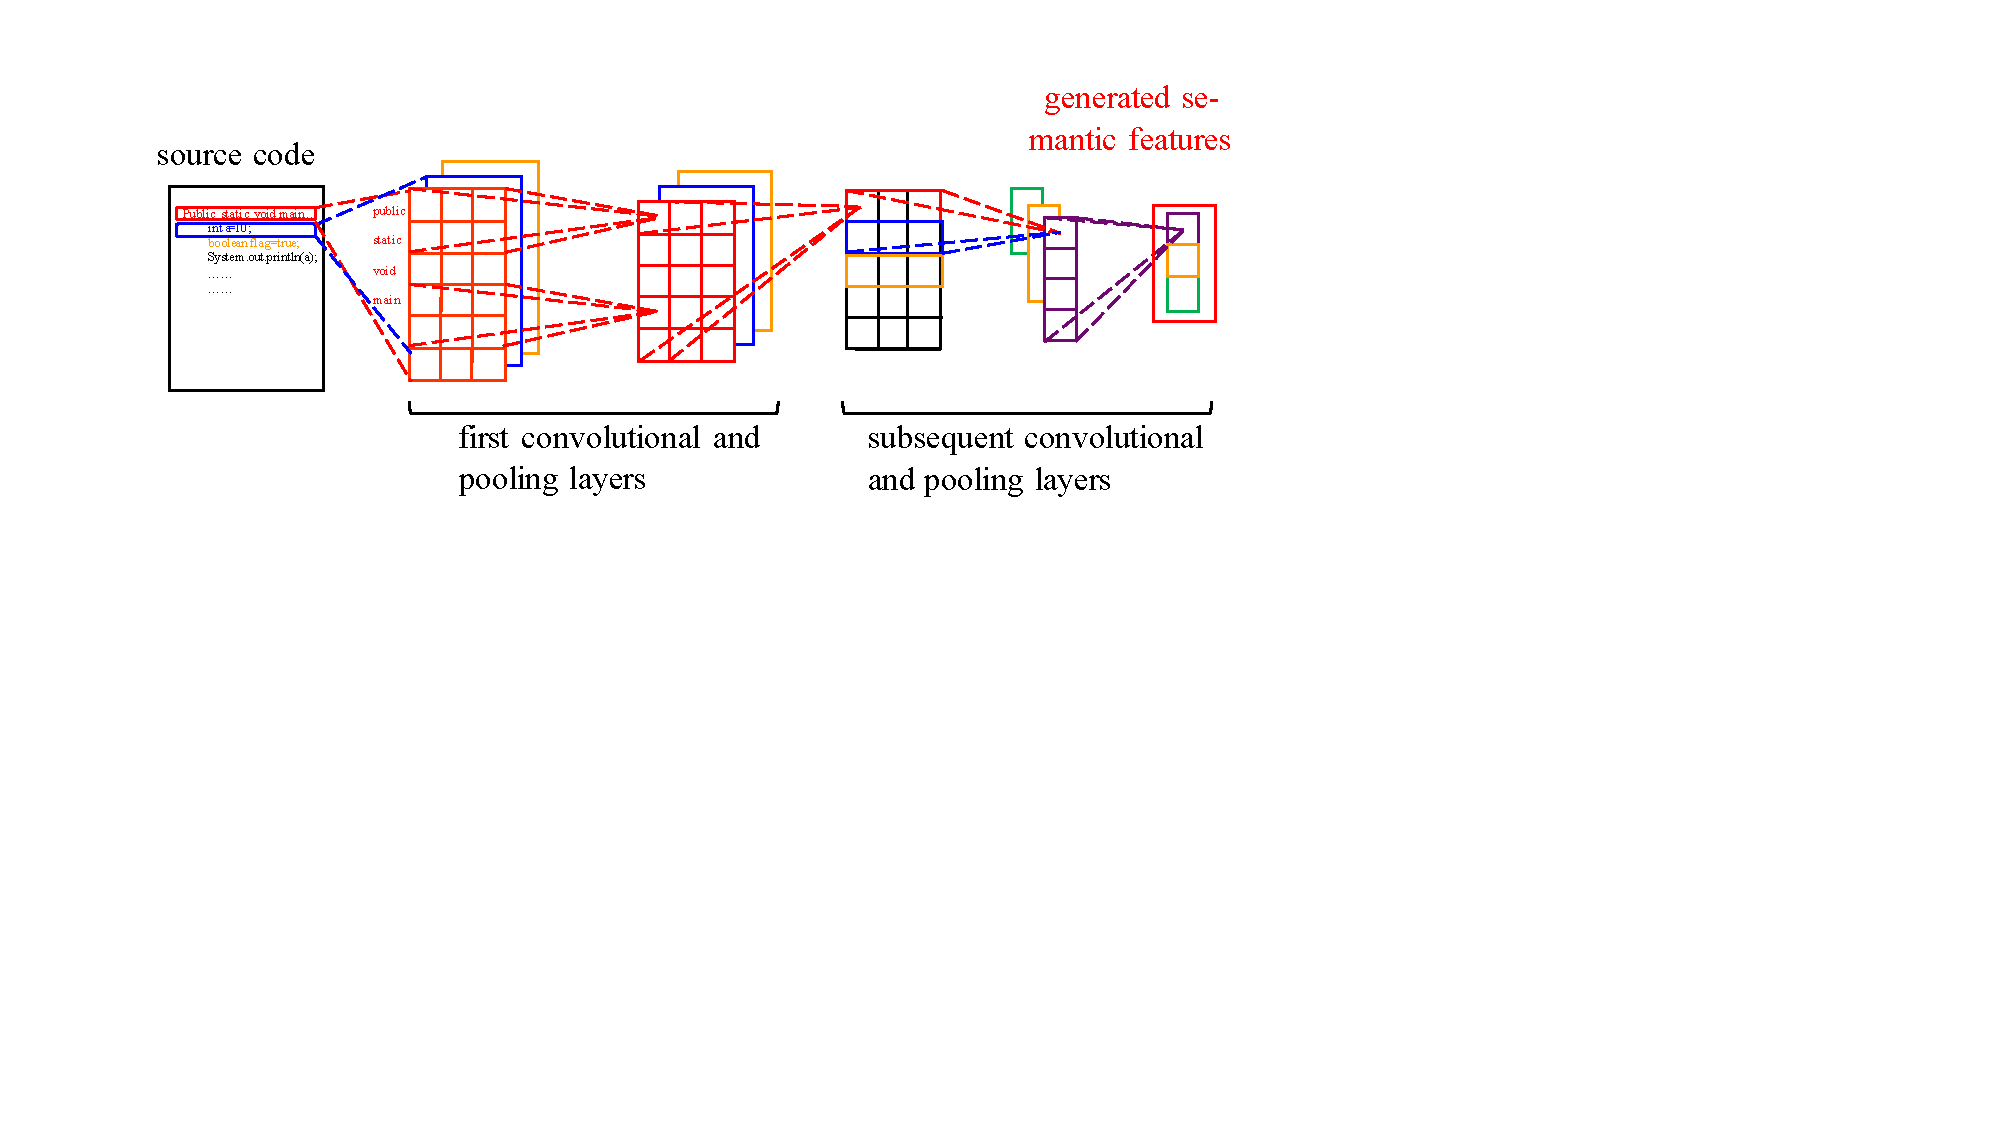
\includegraphics[width = \columnwidth]{pic/NPCNN.pdf}
\caption{The structure of convolutional neural network for programming language.}
\label{fig:npcnn}
\end{figure}

After feature extraction, the middle-level features generated from bug reports and source code are fed into the cross-language feature fusion layers. To deal with the imbalance nature of bug localization data, the cross-language feature fusion layers introduce an unequal misclassification cost according to the imbalance ratio and train the fully connected network in a cost sensitive manner. Let $cost_n$ denotes the cost of incorrectly associating an irrelevant source code file to a bug report and $cost_p$ denotes the cost of missing a buggy source code file that is responsible for the reported bugs. The weights of the fully connected networks $w$ can be learned by minimizing the following objective function using SGD (Stochastic Gradient Descent).
\begin{equation}
\begin{aligned}
\label{eq:cost2}
\mathop{\min}_{\mathbf{w}}\sum_{i,j}{[cost_n L(\mathbf{z}^{r}_i, \mathbf{z}^{c}_j, y_{ij}; \mathbf{w})(1-y_{ij})} \\
 {+cost_p L(\mathbf{z}^{r}_i, \mathbf{z}^{c}_i, y_{ij}; \mathbf{w})(1+y_{ij})]}+\lambda||\mathbf{w}||^2
\end{aligned}
\end{equation}

